\documentclass[10pt]{article}

\usepackage[margin=0.75in]{geometry}
\usepackage{fancyhdr}
\pagestyle{fancy}
\usepackage{amsmath}
\usepackage{amssymb}
\usepackage{color}

\definecolor{mygreen}{rgb}{0,0.6,0}
\definecolor{mygray}{rgb}{0.5,0.5,0.5}
\definecolor{mymauve}{rgb}{0.58,0,0.82}

\usepackage{graphicx}
\usepackage{listings}
\lstset{language=Python,
		keywordstyle=\color{blue},
		commentstyle=\color{mygreen},
		numbers=left,
		numbersep=5pt,
	    numberstyle=\color{mymauve}, % the style that is used for the line-numbers
        rulecolor=\color{green},         
        showspaces=false,                
  		showstringspaces=false,          % underline spaces within strings only
  		showtabs=false,                  % show tabs within strings adding particular underscores
  		stepnumber=1}

\allowdisplaybreaks

\lhead{FEM 5168 HW1}
\chead{Melvyn Ian Drag}
\rhead{\today}
\setlength{\parskip}{0pt} 
\setlength{\parindent}{0pt}
\newcommand{\tab}[1]{\hspace*{4ex}\rlap{#1}}
\newcommand{\tbf}[1]{\textbf{#1}}
\newcommand{\ptl}[2]{\frac{\partial^2 #1}{\partial #2 ^2}}
\newcommand{\der}[2]{\frac{d #1}{d #2}}
\newcommand{\iab}[2]{\int_{ #1 }^{ #2 }}
\begin{document}
\section*{Problem 1}
The weak form is 
\begin{equation*}
\int_0^1(1+x)\der{u}{x}\der{v}{x}dx = \int_0^1vdx. 
\end{equation*}
The piecewise linear basis functions are described on pages 17 and 19 of the lecture 4 notes.
\subsection*{Part a}
\begin{flalign*}
\textbf{K}_{11} &= \int_0^1(1+x)(\phi_1')^2dx\\
&= \int_0^{\frac12}(1+x)(2)^2dx + \int_{\frac12}^{1}(1+x)(-2)^2dx\\
&=4\int_0^1(1+x)dx = 6\\
\tbf{F}_{11} &= \int_0^1 \phi_1dx\\
&=\int_0^{\frac12}2xdx+\int_{\frac12}^{1}2(1-x)dx\\
&= x^2\bigg|_0^{\frac12}+2x-x^2\bigg|_{\frac12}^1\\
&=\frac14+1-(1-\frac14) = \frac12\\
\implies \alpha &=\frac1{12}
\end{flalign*}
\subsection*{Part b}
The vector \tbf{F} is easy to calculate. All of its entries have to be the same since the basis functions are all translations of the first one (the areas they bound are equal). \tbf{F} is a vector with all entries equal to:
\begin{equation*}
\iab{0}{0.25}4xdx + \iab{0.25}{0.5}4(0.5-x)dx = 0.25
\end{equation*}
We again compute the entry $k_{ij}$ of the stiffness matrix as $k_{ij} = \int_0^1(1+x)\phi_i'\phi_j'dx$. We have to break these integrals down into a sum of two integrals to deal with each piece of the basis function. 
\begin{gather*}
k_{11} = \int_0^{0.25}(1+x)(4)^2dx+\iab{0.25}{0.5}(1+x)(-4)^2dx = 16\iab{0}{0.5}(1+x)dx = 16*(0.28125 + 0.34375) = 10\\
k_{12} = \iab{0}{0.25}(1+x)(4)(0)dx + \iab{0.25}{0.5}(1+x)(4)(-4)dx = -16(0.34375) = -5.5\\
k_{13} = \iab{0}{0.25}(1+x)(4)(0)dx + \iab{0.25}{0.5}(1+x)(-4)(0)dx = 0\\
k_{22} = \iab{0.25}{0.5}(1+x)(4)^2dx + \iab{0.5}{0.75}(1+x)(-4)^2dx = 12\\
k_{23} = \iab{0.25}{0.5}(1+x)(4)(0)dx +\iab{0.5}{0.75}(1+x)(-4)(4)dx = -6.5\\
k_{33} = \iab{0.5}{1.0}(1+x)(16)dx = 14
\end{gather*}
\begin{center}
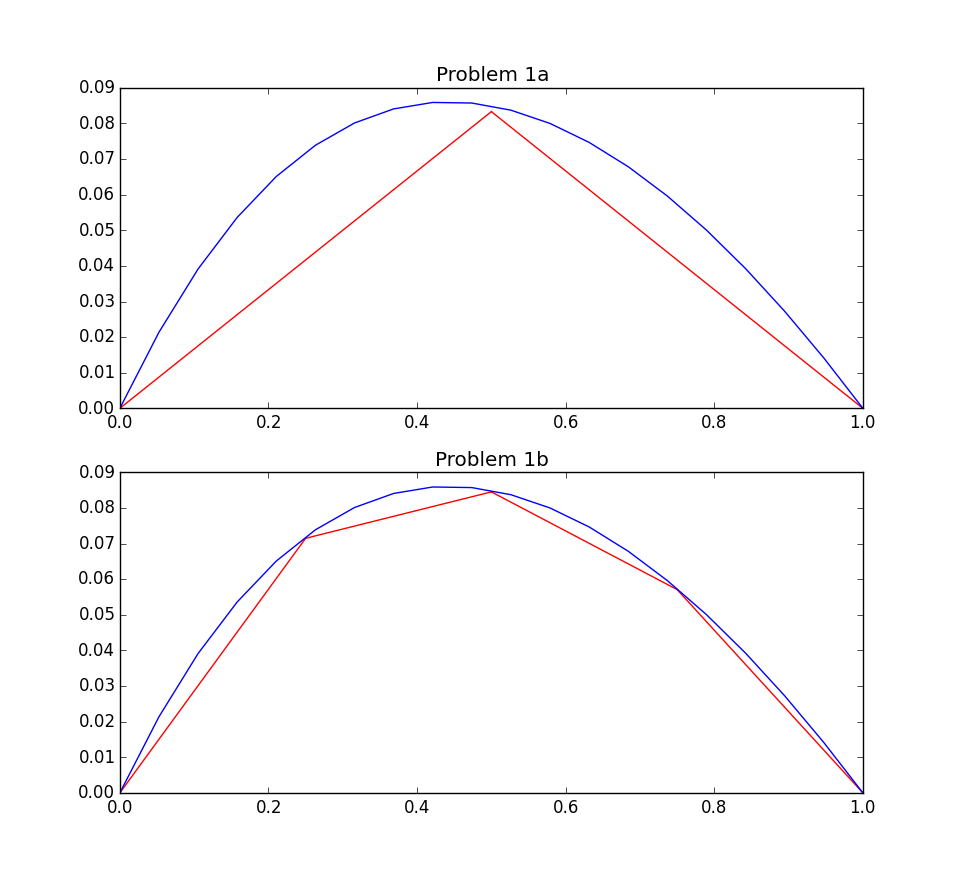
\includegraphics[scale = 0.5]{prob1.png}
\end{center}
\begin{lstlisting}
from numpy import log, linspace, array
from numpy.linalg import solve
import matplotlib.pyplot as plt

# Part A
alpha = 1.0/12.0
el1 = lambda x: 2.0*x
el2 = lambda x: 2.0*(1.0 - x)
u = lambda x: log(1+x)/(log(2))-x

x = linspace(0, 1, 20)
x1 = linspace(0, 0.5, 10)
x2 = linspace(0.5, 1, 10)

plt.subplot(2, 1, 1)
plt.plot(x1, alpha*el1(x1),'r', x2, alpha*el2(x2), 'r', x, u(x), 'b')
plt.title('Problem 1a')

# Part B
K = array([[10, -5.5, 0],[-5.5, 12, -6.5],[0, -6.5, 14]])
f = 0.25
F = array([f, f, f])
alpha =  solve(K,F)

el1 = lambda x: alpha[0]*4*x
el2 = lambda x: alpha[1]*4*(x - 0.25) + alpha[0]*4*(0.5 - x)
el3 = lambda x: alpha[1]*4*(0.75 - x) + alpha[2]*4*(x - 0.5)
el4 = lambda x: alpha[2]*4*(1 - x)
u   = lambda x: log(1+x)/(log(2))-x

x  = linspace(0,1,20)
x1 = linspace(0, 0.25, 10)
x2 = linspace(0.25, 0.5, 10)
x3 = linspace(0.5, 0.75, 10)
x4 = linspace(0.75, 1, 10)

plt.subplot(2, 1, 2)
plt.plot(x1, el1(x1), 'r', x2, el2(x2), 'r', x3, el3(x3), 'r', x4, el4(x4), 'r', x, u(x), 'b')
plt.title('Problem 1b')
plt.show()
\end{lstlisting}
\section*{Problem 2}
For the cubic master element we need four nodes over an interval, and for convenience we use $[-1, 1]$. This gives us the nodes: $\xi_1 = -1,\; \xi_2= -\frac13,\;\xi_3=\frac13,\;\xi_4=1.$
Then, the Lagrange shape functions are given by:
\begin{gather*}
f(\xi, \xi_i) = \frac{(\xi - \xi_1)...(\xi-\xi_{i-1})(\xi - \xi_{i+1})...(\xi - \xi_n)}{(\xi_i - \xi_1)...(\xi_i-\xi_{i-1})(\xi_i - \xi_{i+1})...(\xi_i - \xi_n)}\\
\psi_i = f(\xi, \xi_i), \;\; n = 4 \\
\psi_1 = -\frac{9}{16}x^3+\frac{9}{16}x^2 + \frac x{16} - \frac1{16}\\
\psi_2 = \frac{27}{16}x^3 - \frac{9}{16}x^2-\frac{27}{16}x+\frac9{16}\\
\psi_3 = -\frac{27}{16}x^3-\frac9{16}x^2+\frac{27}{16}x+\frac9{16}\\
\psi_4 = \frac9{16}x^3+\frac9{16}x^2-\frac x{16}-\frac1{16}
\end{gather*}

\begin{center}
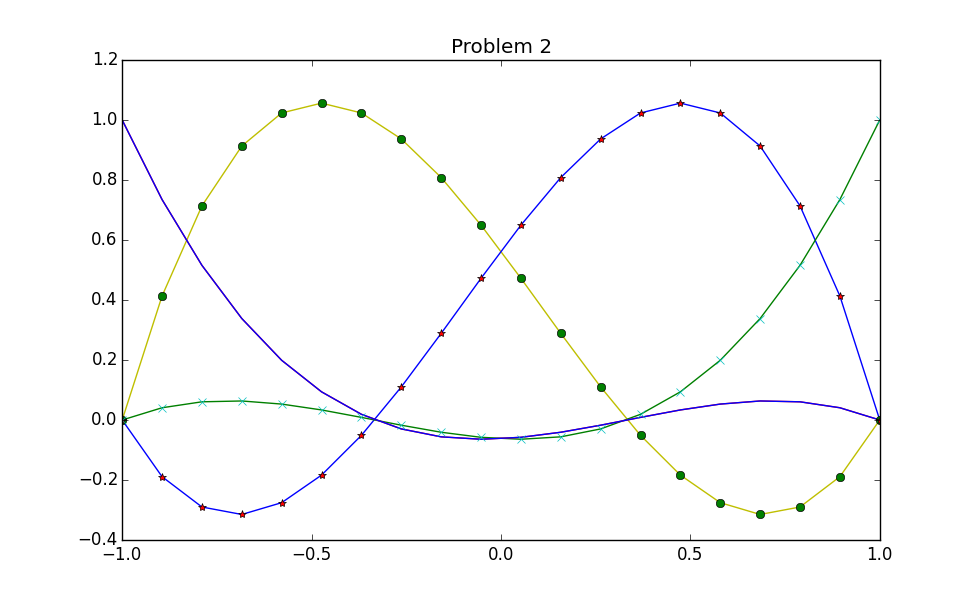
\includegraphics[scale = 0.7]{prob2.png}
\end{center}

\section*{Problem 3}

\begin{lstlisting}
function psi = lagrange_poly(k)
%{
k is the degree of the basis functions.
The general structure of this code is:
1) Set some necessary variables.
2) To make the coefficients we first convolute the numerator terms in the 
   expression for the lagrange polynomial.
   Then, we multiply the denominator terms and multiply the denominator
   by the coefficient array. 
   We have to go through this for each basis function.
3) Store the basis functions and their derivatives.
%}

xi_m = -1; % minimum xi
xi_M =  1; % maximum xi
xi = linspace(xi_m, xi_M, k+1); % generate k+1 nodes.

for func=1:k+1
    
    % Initialize identity elements.
    f = [1];
    denom = 1;
    
    % In this loop we will multiply the numerator and denominator factors.
    for factor = 1:k+1
        if (factor ~= func)
            f = conv(f, [1, -xi(factor)]);
            denom = denom * (xi(func) - xi(factor)); 
        end
    end
    
    % Set the basis function and its derivative.
    F = f/denom;
    psi(func).fun = F;
    power_rule = [k:-1:0];
    dF = F.*power_rule;          % Apply power rule.
    psi(func).der = dF(1:end-1); % Trim off end 0 element.

end
\end{lstlisting}
\end{document}